\section{VEX 393 Alternative Motor Gearing}

\begin{figure}[h]
    \centering
    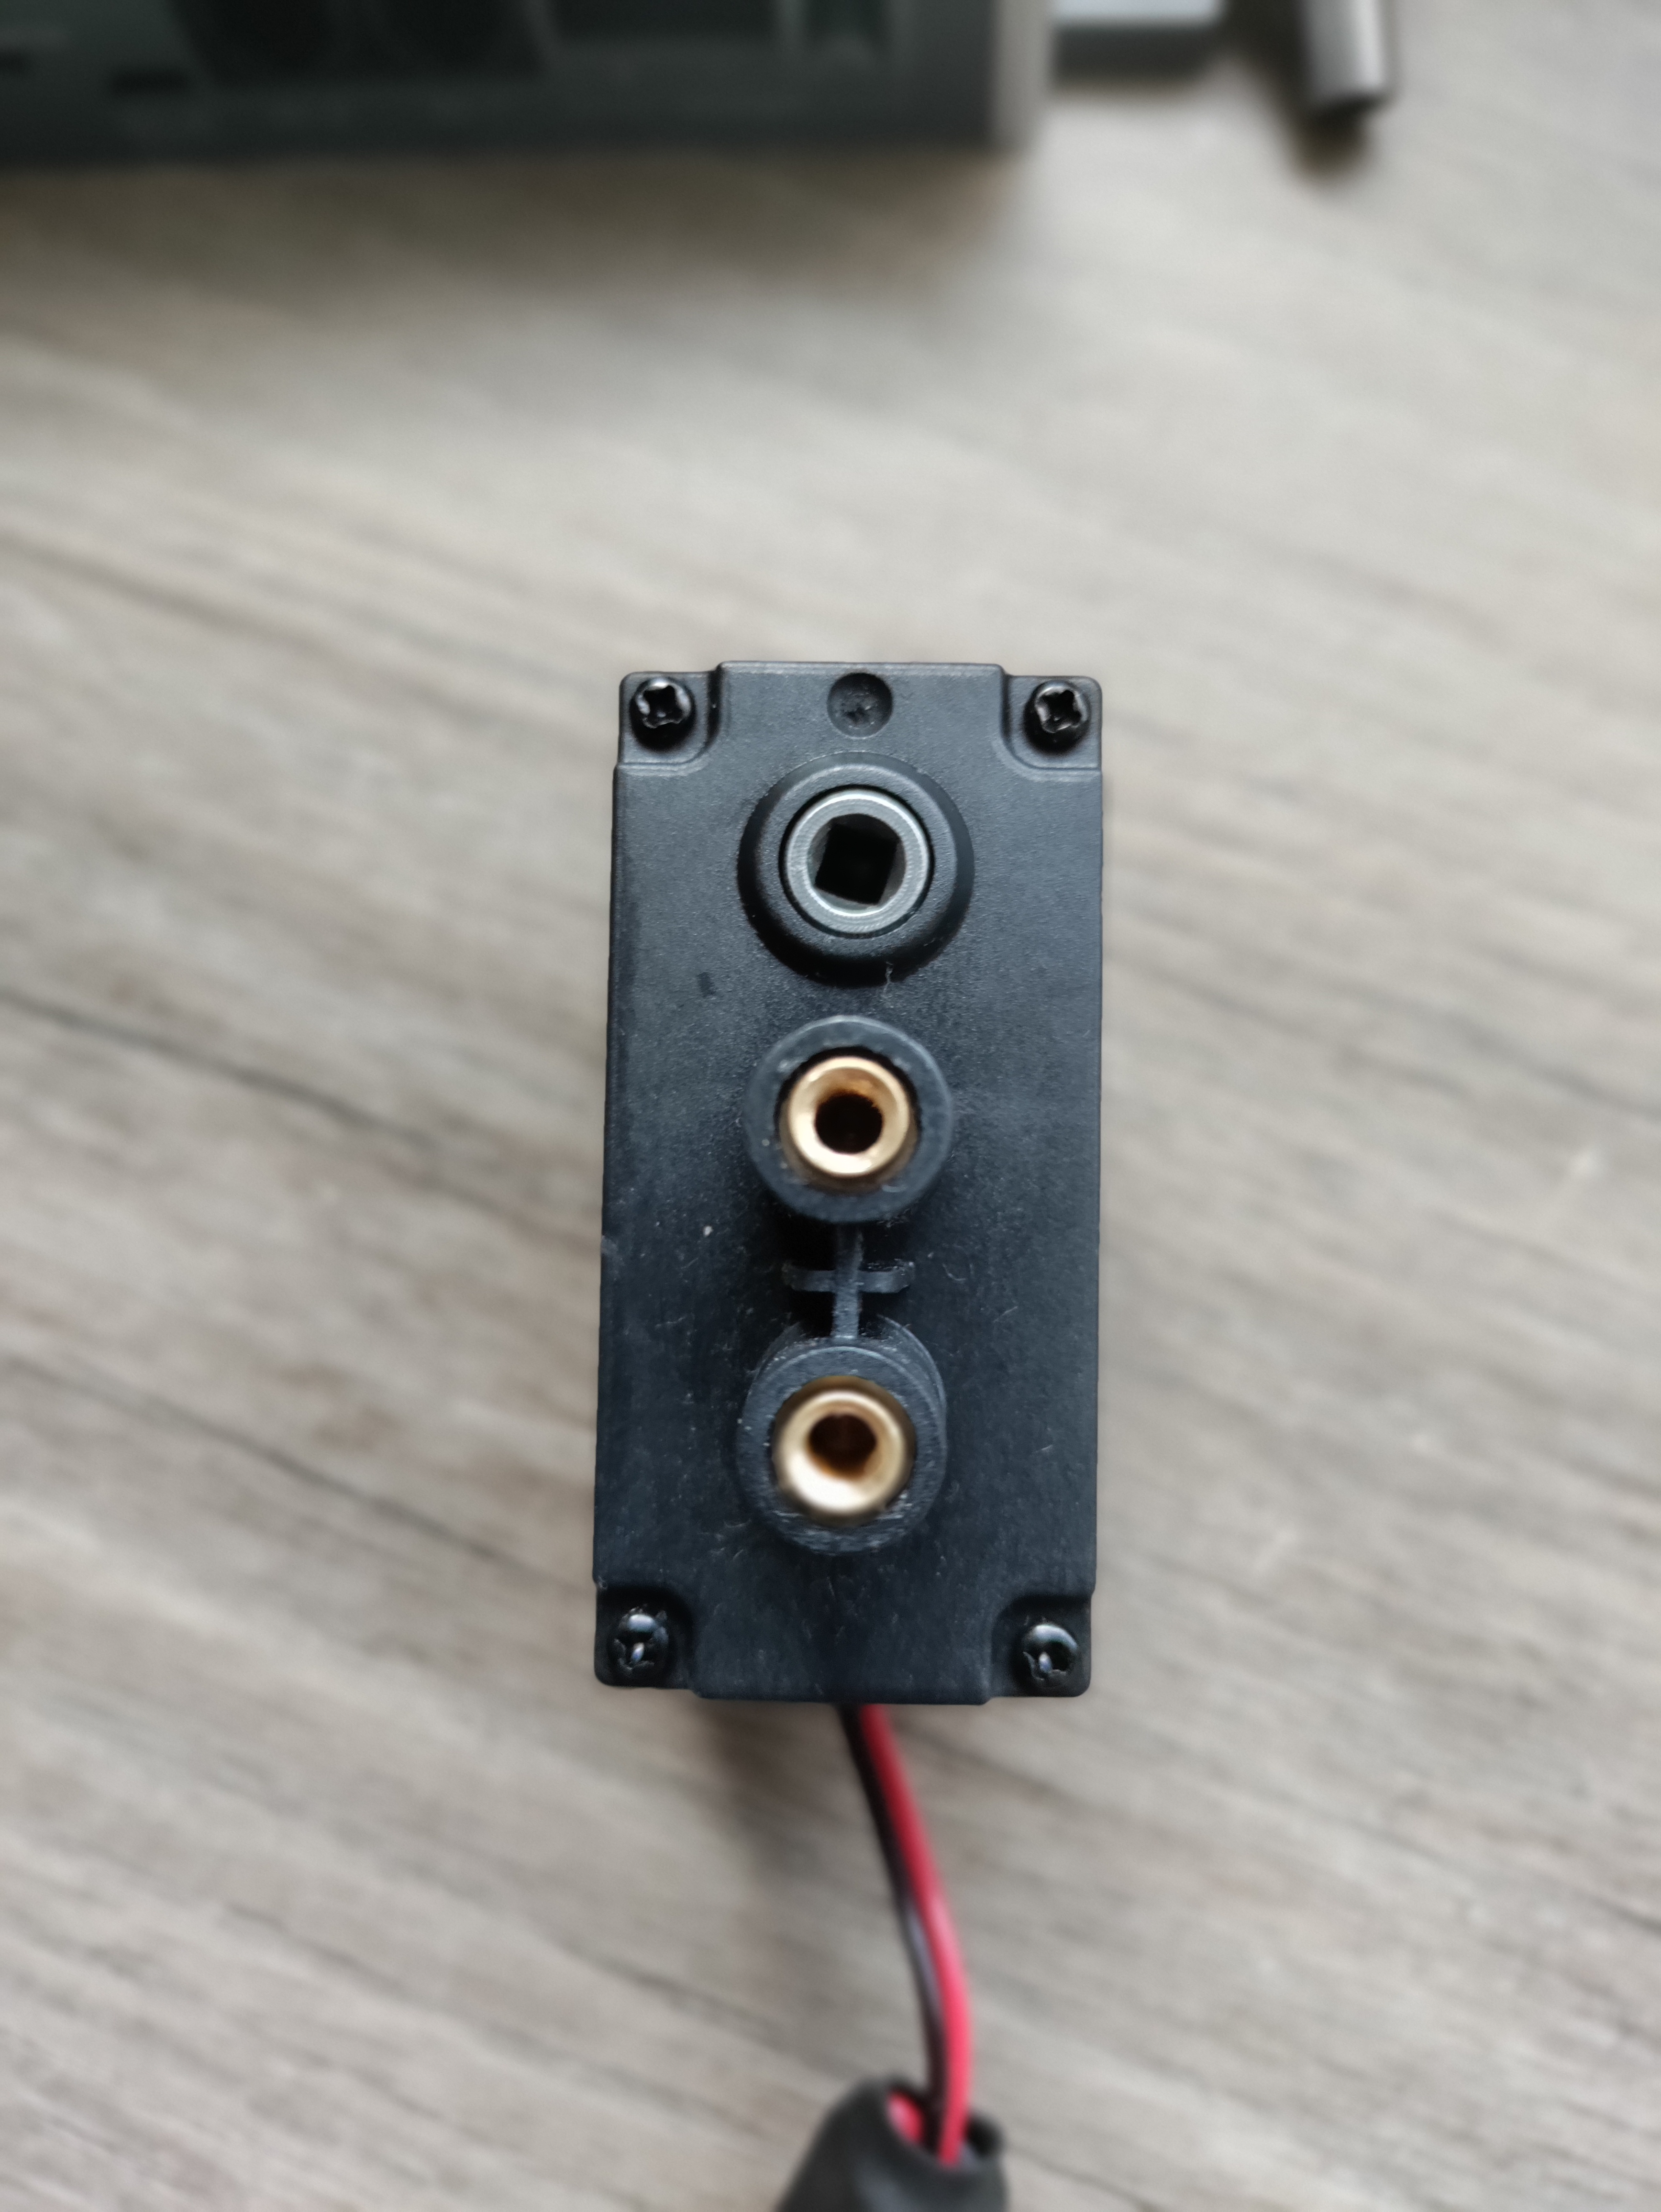
\includegraphics[width=\textwidth,height=9cm,keepaspectratio=true]{MotorGearing/MotorAssembled}
    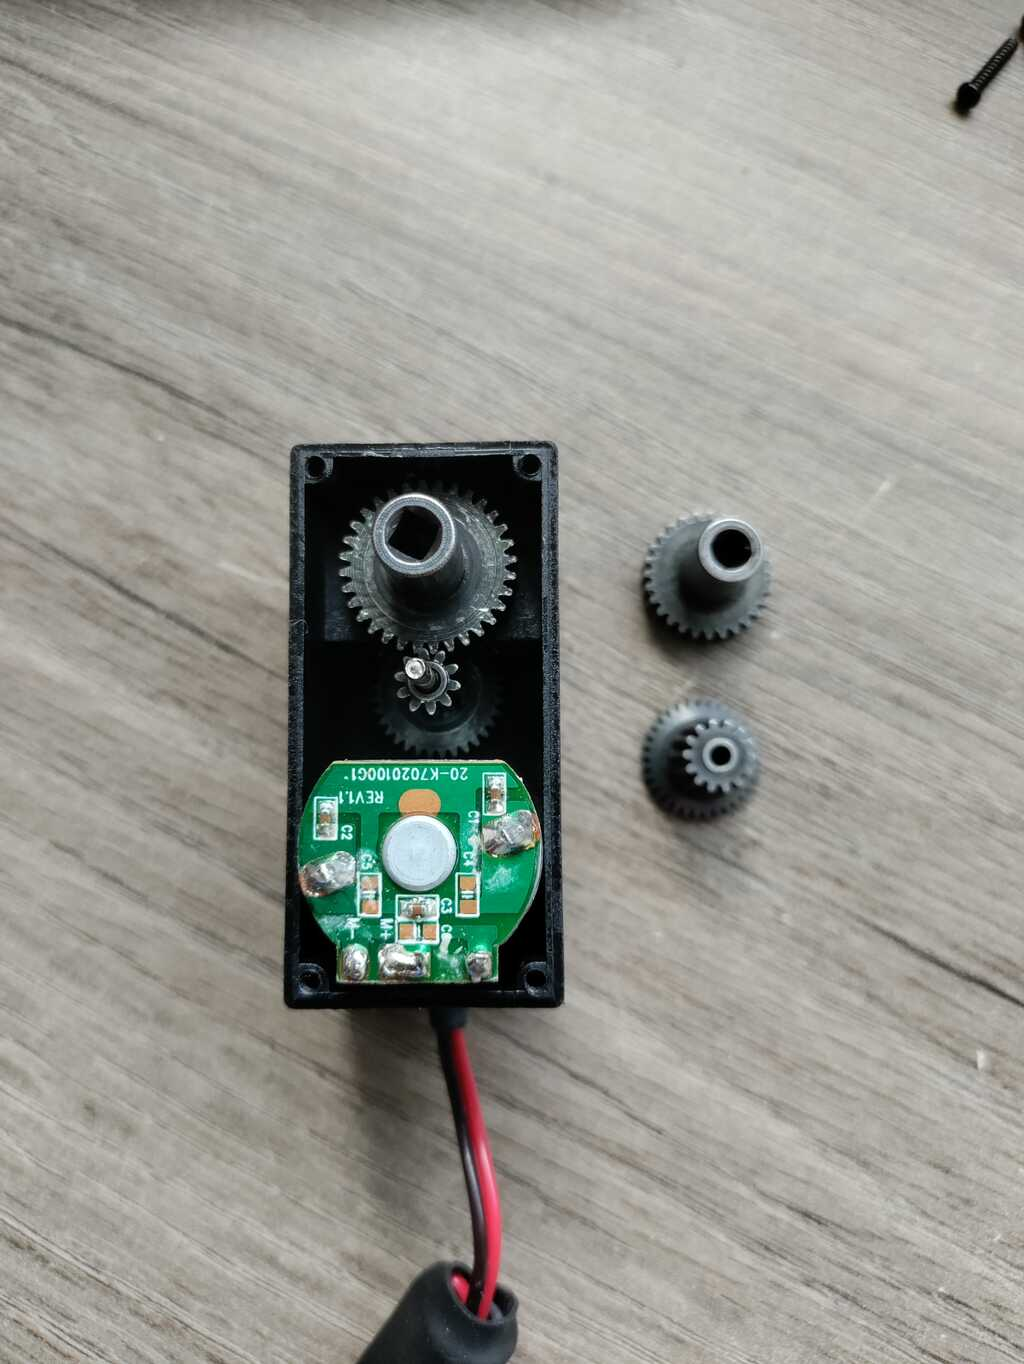
\includegraphics[width=\textwidth,height=9cm,keepaspectratio=true]{MotorGearing/MotorDisassembled}
    \caption{
        (Left) The front portion of the motor; This is the only thing you should unscrew. (Right) The regular motor gearing with the high-speed option gears. Notice how it has a different ratio.
    }
\end{figure}

Our VEX Classroom Kit comes with extra metal gears for motors; Some are merely replacement parts, and others change the gear ratio. By unscrewing the portion of the motor that attaches to an axle, you reveal two gears that can be removed. If you replace these gears with the high-speed version of those gears, you can increase the speed of the motors by 60\% while reducing torque by 60\% \cite{VEXMotor}. With this, you can make a higher speed chassis without worring about attaching other gears, thus saving time. If our kit contained the VEX Turbo Gear Set, this percentage goes up to 240\% \cite{VEXMotor}, which is ridiculous.
